% *********************************************************************
% © 2010–2021 Jeremy Sylvestre
%
% Permission is granted to copy, distribute and/or modify this document
% under the terms of the GNU Free Documentation License, Version 1.3 or
% any later version published by the Free Software Foundation; with no
% Invariant Sections, no Front-Cover Texts, and no Back-Cover Texts. A
% copy of the license is included in the appendix entitled “GNU Free
% Documentation License” that appears in the output document of this
% PreTeXt source code. All trademarks™ are the registered® marks of
% their respective owners.
%
% *********************************************************************

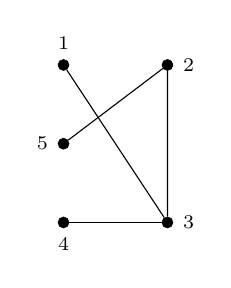
\begin{tikzpicture}[
	xscale=0.66,
	vertex/.style={ circle, draw, very thin, fill, inner sep=0pt, minimum size=4pt },
	vertexg/.style={ black!40!white, circle, draw, very thin, fill, inner sep=0pt, minimum size=4pt },
	vertexo/.style={ circle, draw, very thin, inner sep=0pt, minimum size=4pt }
]

\node at (0,2) (one) [vertex,label=above:$\scriptstyle 1$] {};
\node at (2,2) (two) [vertex,label=right:$\scriptstyle 2$] {};
\node at (2,0) (three) [vertex,label=right:$\scriptstyle 3$] {};
\node at (0,0) (four) [vertex,label=below:$\scriptstyle 4$] {};
\node at (0,1) (five) [vertex,label=left:$\scriptstyle 5$] {};

\draw (two) to (three) to (one);
\draw (four) to (three);
\draw (five) to (two);

\end{tikzpicture}
